\def \path {misc/dtcwt_proofs}
\def \imgpath {\path/images}

\section{Complex Convolution and Gradients}

Consider a complex number $z=x+iy$, and the complex mapping 

$$w=f(z) = u(x,y) + iv(x,y)$$ 

where $u$ and $v$ are called `conjugate functions'. Let us examine the
properties of $f(z)$ and its gradient. 

The definition of gradient for complex numbers is:

$$ \lim_{\Delta z\to 0} \frac{f(z + \Delta z) - f(z)}{\Delta z}$$

A necessary condition for $f(z,\conj{z})$ to be an analytic function is
$\dydx{f}{\conj{z}}=0$. I.e.\ f must be purely a function of $z$, and not
$\conj{z}$.

A geometric interpretation of complex gradient is shown in
\autoref{fig:complex_grad}.  As $\Delta z$ shrinks to 0, what does $\Delta w$
converge to? E.g.\ consider the gradient of approach $m=\frac{dy}{dx}=\tan
\theta$, then the derivative is

$$\gamma = \alpha + i\beta = D(x,y) + P(x,y)e^{-2i\theta}$$

where

\begin{eqnarray*}
  D(x,y) & = & \half(u_x + v_y + i(v_x - u_y)) \\
  P(x,y) & = & \half(u_x - v_y + i(v_x + u_y))
\end{eqnarray*}

$P(x,y)=\frac{dw}{d\conj{z}}$ needs to be 0 for the function to be analytic.
This is where we get the Cauchy-Riemann equations:

$$\dydx{u}{x}= \dydx{v}{y}$$ 
and 
$$\dydx{u}{y}= -\dydx{v}{x}$$ 

The function $f(z)$ is analytic (or regular or holomorphic) if the derivative 
$f'(z)$ exists at all points z in a region $R$. If $R$ is the entire z-plane,
then f is entire. 

\begin{figure}[!h]
	\centering
  \subfloat{%
	\begin{tikzpicture}[>=latex,scale=0.6]
	\draw[style=help lines, color=gray!30, dashed] (-4.9,-4.9) grid[step=1cm] (4.9,4.9);
	\draw[->,ultra thick] (-5,0)--(5,0) node[right]{$x$};
	\draw[->,ultra thick] (0,-5)--(0,5) node[above]{$y$};

	\coordinate (z) at (20:4); % Define some complex numbers
	\coordinate (dz) at (100:1); % with r*exp(i \theta) form

	\draw[->,thick,blue] (0,0) -- (z) node[near end,below=-0.05] {$z$};
	\draw[->,thick,red] (z)  -- ++(dz) node[near end,right] {$\Delta z$};
	\draw[->,thick,green] (0,0) -- ($(z) + (dz)$) node[near end,above left] {$z+\Delta z$};
	\node[above,font=\large] at (current bounding box.north) {z-plane};
	\end{tikzpicture}
}
\subfloat{%
	\begin{tikzpicture}[>=latex,scale=0.6]
	\draw[style=help lines, color=gray!30, dashed] (-4.9,-4.9) grid[step=1cm] (4.9,4.9);
	\draw[->,ultra thick] (-5,0)--(5,0) node[right]{$x$};
	\draw[->,ultra thick] (0,-5)--(0,5) node[above]{$y$};

	\coordinate (w) at (-30:4); % Define some complex numbers
	\coordinate (dw) at (20:1); % with r*exp(i \theta) form

	\draw[->,thick,blue] (0,0) -- (w) node[near end,below] {$w$};
	\draw[->,thick,red] (w) -- ++(dw) node[near end,below] {$\Delta w$};
	\draw[->,thick,green] (0,0) -- ($(w) + (dw)$) node[near end, above=0.1] {$w+\Delta w$};
	\node[above,font=\large] at (current bounding box.north) {w-plane};
	\end{tikzpicture}
}

  \mycaption{Geometric interpretation of complex gradient}{The gradient is
  defined as $f'(z) = \lim_{\Delta z \to 0} \frac{\Delta w}{\Delta z}$. It must
  approach the same value independent of the direction $\Delta z$ approaches
  zero. This turns out to be a very strong and somewhat restrictive property.}
  \label{fig:complex_grad}
\end{figure}




\subsubsection*{Grad Operator}
Recall, the gradient is a multi-variable  generalization of the derivative. The
gradient is a vector valued function. In the case of complex numbers, it can be
represented as a complex number too. E.g.\ consider $W(z) = F(x,y)$ (note that
in general it may be simple to find F given G, but they are different
functions).

I.e. 
$$\nabla F = \dydx{F}{x} + i \dydx{F}{y}$$

Consider the case when F is purely real, then 
$F(x,y) = F(\frac{z+\conj{z}}{2},\frac{z-\conj{z}}{2i}) = G(z,\conj{z})$
Then
$$\nabla F = \dydx{F}{x} + i \dydx{F}{y} = 2\dydx{G}{\conj{z}}$$

If F is complex, let $F(x,y) = P(x,y) + iQ(x,y) = G(z,\conj{z})$, then
$$\nabla F = \left(\dydx{}{x} + i \dydx{}{y}\right)(P+iQ) 
           = \left(\dydx{P}{x} - \dydx{Q}{x}\right) + 
                i\left(\dydx{P}{y} + \dydx{Q}{x}\right) 
           = 2\dydx{G}{\conj{z}}$$
It is clear to see how the purely real case is a subset of this (set Q=0 and
all its partials will be 0 too).

If G is an analytic function, then $\dydx{G}{\conj{z}} = 0$ and so the gradient
is 0, and the Cauchy-Riemann equations hold $\dydx{P}{x}=\dydx{Q}{y}$ and 
$\dydx{P}{y}=-\dydx{Q}{x}$

\subsubsection*{Hilbert Pairs of General Functions}
  How does this affect me? I don't think I'll be able to use analytic
  non-linearities, however I may be able to have analytic filters, like those of
  the \DTCWT.

  The Hilbert pair of the cosine is the sine function, but what about in general?
  If $x=\delta(t)$, its Hilbert pair $jy = \frac{-j}{\pi t}$. Like the dirac
  delta function, this also has a flat spectrum, and the figure for it is shown
  below.

  \begin{center}
    \begin{tikzpicture}[scale=0.6]
  \draw[->] (-4,0) -- (4,0) node[right] {$x$};
  \draw[->] (0,-4) -- (0,4) node[above] {$y$};
   \draw[domain=-4:-0.1,smooth,variable=\x,blue] 
     plot ({\x},{1/(pi*\x)});
   \draw[domain=0.1:4,smooth,variable=\x,blue] 
     plot ({\x},{1/(pi*\x)});
\end{tikzpicture}

  \end{center}

  That means if we wanted to get the Hilbert pair of a sampled signal, then we
  would have to add shifts and scales of $y$, which unfortunately has infinite
  support. We would also have to lowpass it, as we do for the sampled version
  (so their frequency spectrums are the same).

\subsubsection*{Usefulness of Complex Numbers}
  Nick made a good point in our recent meeting that when trying to use the
  complex plane, we must know/understand what it is we want to gain from the
  added representation. For the case of the \DTCWT, he converted the non-analytic
  sinusoids of the wavelet transform into an analytic signal.

  I.e.\ let us ignore the previous notation of $x=\Re(z), y=\Im(z)$ and redefine
  them to indicate the horizontal and vertical directions in an image.

  For a real wavelet transform, all of the cosine terms are
  $$\cos \omega_1 x = \half\left(e^{j\omega_1 x} + e^{-j\omega_1 x} \right)$$
  If we consider $z_x = e^{j\omega_1 x}$, then this is clearly a function of both
  $z_x$ and its conjugate (as are all real valued functions). I.e. $\cos \omega_1
  x = F(z_x,\conj{z_x})$. Nick replaced this with the analytic equivalent of this
  function by adding in the Hilbert pair term.
  $$\cos \omega_1 x +j \sin \omega_1 x = e^{j\omega_1 x} = F(z_x)$$
  From our above definitions of analytic functions, it is clear to see that this
  is now no longer a function of the conjugate term $\conj{z_x}$, so it is analytic. The
  benefit for Nick was that now he could separably multiply the x and the
  y sinusoids to get:
  $$e^{j\omega_1 x} \times e^{j\omega_2 y} =F(z_x)F(z_y)= e^{j(\omega_1 x + \omega_2 y)}
  = F(z_x+z_y)$$

  Also, I must be careful with regularizing complex weights. We want to set some
  of the weights to 0, and let the remaining ones evolve to whatever phase they
  please. To do this, either use the L-2 norm on the real and imaginary parts
  independently, or be careful about using the L-1 norm. This is because we
  really want to be penalising the magnitude of the complex weights, $r$ and: 
  $$\lnorm{r}{2}^2 = \lnorm{\sqrt{x^2+y^2}}{2}^2 = \sum x^2 + y^2 = \sum x^2 + \sum y^2
  = \lnorm{x}{2}^2 + \lnorm{y}{2}^2$$
  But this wouldn't necessarily be the case for the L-1 norm case.

\section*{Working with Complex weights in CNNs}
  As a first pass, I think I shouldn't concern myself too much with analytic
  functions and having the Cauchy-Riemann equations met. Instead, I will focus
  on implementing the CNN with a real and imaginary component to the filters,
  and have these stored as independent variables.\\\\
  Unfortunately, most current neural network tools only work with real numbers,
  so we must write out the equations for the forward and backwards passes, and
  ensure ourselves that we can achieve the equivalent of a complex valued
  filter.
\subsection*{A review of what we have done so far}
  This was inspired by our recent work with creating 12 tap complex filters
  that worked across the 6 \DTCWT\ orientations (and their complex conjugate).
  We found that having symmetric filters, with a $90\degs$ offset between
  taps created a nice corner like object. In fact, we could then shift these
  filters along to the next coefficients and the output would rotate by
  $30\degs$ (as we'd simply used the next set of wavelet coefficients).\\\\
  Let us give a concrete example. Consider the 4 tap filter:
  $$\left[1, j, j, 1\right]$$
  Now consider the result of doing a forward transform on a $N\x N$ sized
  image. The highpass outputs (let us call them Yh) have size $2^{-k}N \x 2^{-k}N \x 6$ for each
  scale, k.
  When we  put the above filter into the first 4 \DTCWT\ coefficients at
  the same spatial position $(x,y)$ at given scale, $k$ i.e.\
  \begin{lstlisting}
  Yh[k][y,x,0] = 1
  Yh[k][y,x,1] = j
  Yh[k][y,x,2] = j
  Yh[k][y,x,3] = 1
  \end{lstlisting}
  and then do the inverse \DTCWT\, we get the result shown in
  \autoref{fig:one_corner}. Doing this is equivalent to the deconvolution of
  Zeiler and Fergus. What we're really seeing in \autoref{fig:one_corner} is
  the input shape that would give the highest response if we applied a \DTCWT
  to it, and then applied the above filter across the orientations.

  \begin{figure}[!h]
    \centering
    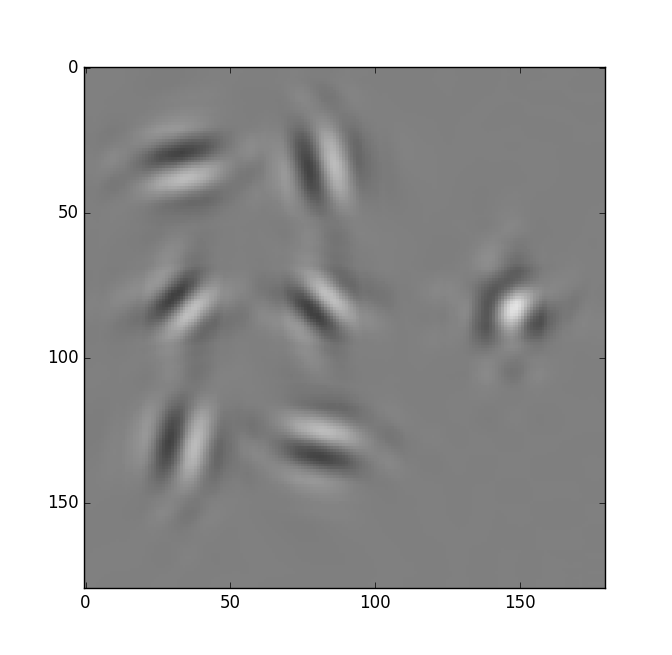
\includegraphics[scale=0.6]{\imgpath/simple_corner.png}
    \caption{Left of image shows the imaginary part of 6 \DTCWT\ impulse responses. Right of image
             shows the effect of combining with the filter $\left[1, j, j,
             1\right]$}
    \label{fig:one_corner}
  \end{figure}

  If we were now to expand our definition of the above filter to be:
  $$\bmu{f} = [1, j, j, 1, 0, 0, 0, 0, 0, 0, 0, 0]$$
  and denote the circular shift of $f$ by k poistions to be $f_k$, then the
  output from shifting f through all 12 positions is shown in
  \autoref{fig:all_corners}. In particular, it is the first shape rotated by
  $30\degs$ for each k.

  \begin{figure}[!h]
    \centering
    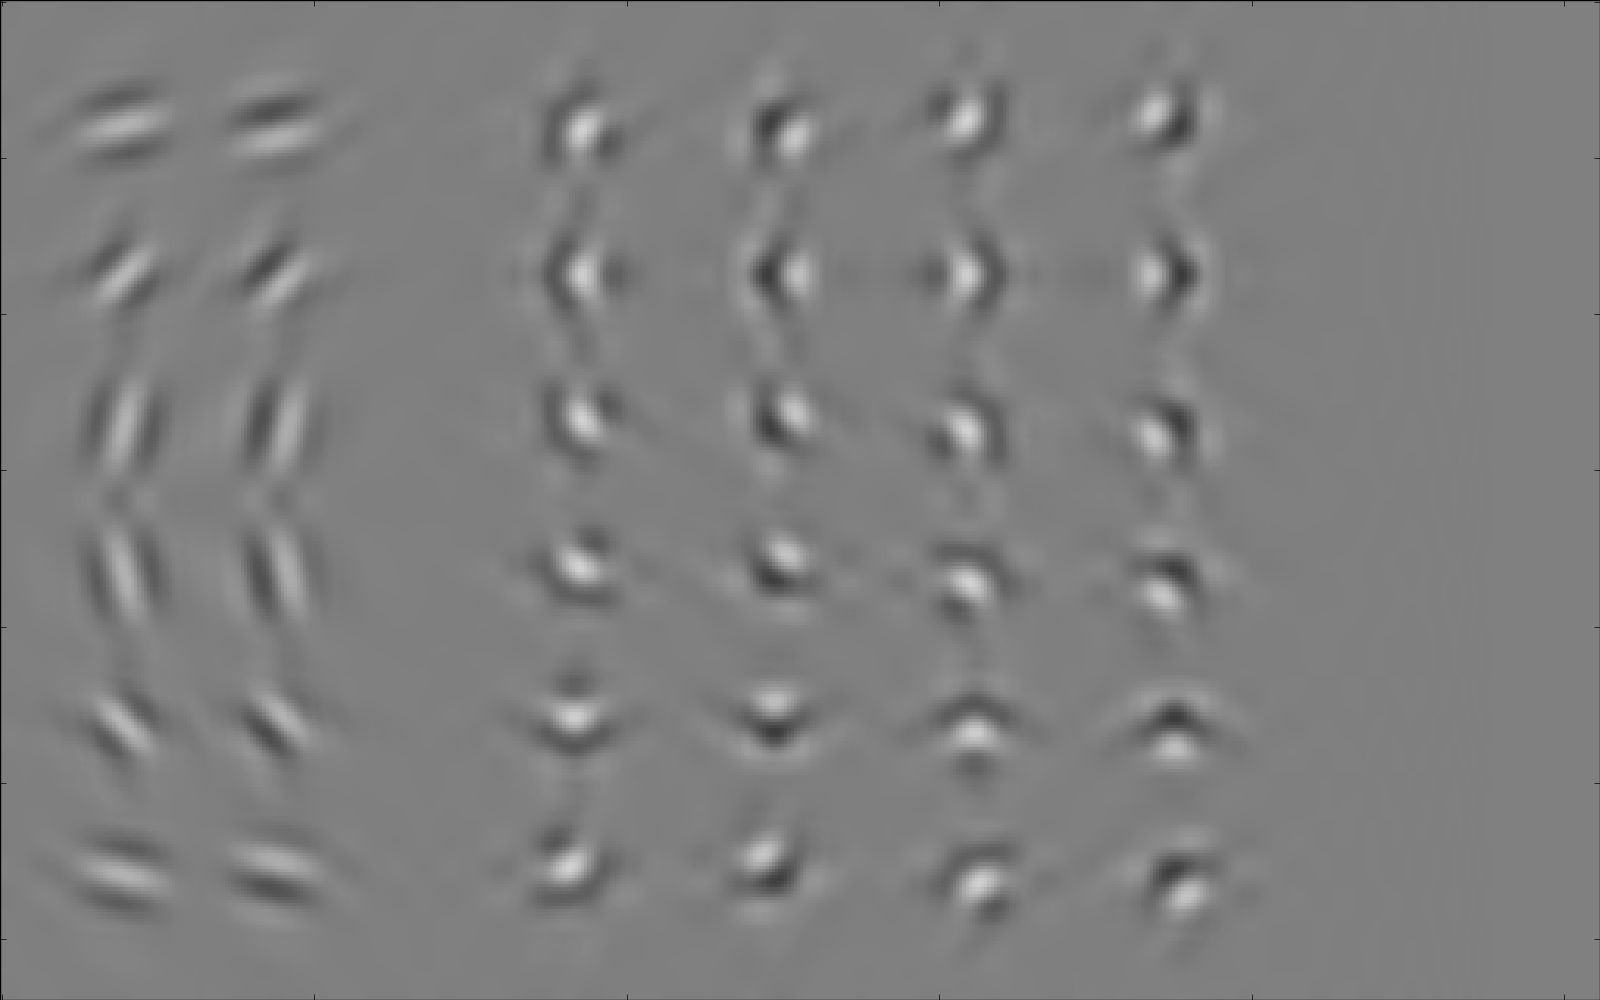
\includegraphics[scale=0.35]{\imgpath/corners_nocross.png}
    \caption{Left shows the 6 real and imaginary \DTCWT\ impulse responses.
    Right of image shows the resulting 12 corners achieved from rotating
    $\left[1, j, j, 1\right]$ through the 12 of these. The even columns are the
    `Hilbert pair' of the odd columns, obtained by shifting all the
    coefficients by $90\degs$ (i.e.\ $\left[j,-1,-1,j\right]$).}
    \label{fig:all_corners}
  \end{figure}
  
\subsection*{Forward pass}
\subsubsection*{Convolution}
  %% Define the variables we will use in this section
  \renewcommand{\SigIn}{\ensuremath{z}\xspace}
  \renewcommand{\SigOut}{\ensuremath{w}\xspace}
  \renewcommand{\Filter}{\ensuremath{f}\xspace}
  \renewcommand{\SigInB}{\ensuremath{\bmu{\SigIn}}\xspace}
  \renewcommand{\SigOutB}{\ensuremath{\bmu{\SigOut}}\xspace}
  \renewcommand{\FilterB}{\ensuremath{\bmu{\Filter}}\xspace}
  %% Now the body
  
  In the above example \FilterB has a spatial support of only $1\x 1$. We still
  were able to get a somewhat complex shape by shifting the relative phases of
  the complex coefficients, but we are inherently limited (as we can only
  rotate the coefficient by at most $2\pi$). So in general, we want to be able
  to consider the family of filters $\FilterB \in \complexes[m_1 \x m_2 \x C]$. For
  ease, let us consider only square filters of spatial support $m$, so
  $\FilterB \in \complexes[m\x m\x C]$. Note that we have restricted the third
  dimension of our filter to be $C=12$ in this case. This means that convolution is
  only in the spatial domain, rather than across channels. Ultimately we would
  like to be able to handle the more general case of allowing the filter to
  rotate through channels, but we will tackle the simpler problem 
  first\footnote{Recall from \autoref{fig:all_corners}, the benefit of allowing
  a filter to rotate through the channel dimension was we could easily obtain
  $30\degs$ shifts of the sensitive shape.}

  Let us represent the complex input with $\SigIn$, which is of shape
  \complexes[n_1\x n_2\x C]. We call \SigOut the result we get from convolving
  \SigInB with \FilterB, so $\SigOutB \in \complexes[n_1 + m - 1, n_2 + m -1, 1]$. With
  appropriate zero or reflective padding, we can make \SigOut have the same
  spatial shape as \SigInB. Now, consider the full complex convolution to get
  \SigOut:
  $$ \SigOut[l_1,l_2] = \sum_{c=0}^{C-1} \sum_{k_1,k_2}
  \Filter[k_1,k_2,c] \SigIn[l_1-k_1,l_2-k_2,c]$$
  Let us define 
  \begin{eqnarray*}
    \SigIn & = & \SigIn_R +j\SigIn_I \\
    \SigOut & = & \SigOut_R +j\SigOut_I \\
    \Filter & = & \Filter_R + j\Filter_I
  \end{eqnarray*}
  where all of these belong to the real space of the same dimension as their
  parent. Then
  \begin{eqnarray*}
    \SigOut[l_1, l_2] & = &  \SigOut_R +j\SigOut_I \\
        & = &\sum_{c=0}^{C-1} \sum_{k_1,k_2} \Filter[k_1,k_2,c] \SigIn[l_1-k_1,l_2-k_2,c]\\
        & = &\sum_{c=0}^{C-1} \sum_{k_1,k_2} (\Filter_R[k_1,k_2,c] +j\Filter_I[k_1,k_2,c]) 
          (\SigIn_R[l_1-k_1,l_2-k_2,c]+ j\SigIn_I[l_1-k_1,l_2-k_2,c])\\
        & = & \sum_{c=0}^{C-1} \sum_{k_1,k_2} (
            \SigIn_R[l_1-k_1,l_2-k_2,c] \Filter_R[k_1,k_2,c] - 
            \SigIn_I[l_1-k_1,l_2-k_2,c] \Filter_I[k_1,k_2,c]) \\
        & +& j\sum_{c=0}^{C-1} \sum_{k_1,k_2} (\SigIn_R[l_1-k_1,l_2-k_2,c] \Filter_I[k_1,k_2,c] + 
            \SigIn_I[l_1-k_1,l_2-k_2,c] \Filter_R[k_1,k_2,c]) \\
        &=& \left((\SigIn_R \ast \Filter_R) - (\SigIn_I \ast \Filter_I)\right)[l_1,l_2] + 
            \left((\SigIn_R \ast \Filter_I) + (\SigIn_I \ast \Filter_R)\right)[l_1,l_2]
  \end{eqnarray*}
  Unsurprisingly, complex convolution is then the sum and difference of 4 real convolutions.

\subsubsection*{Non-Linearity}
  %% Define the variables we will use in this section
  \renewcommand{\SigIn}{\ensuremath{w}\xspace}
  \renewcommand{\SigOut}{\ensuremath{y}\xspace}
	\tdplotsetmaincoords{70}{105}

	\begin{figure}[!h]
    \centering
    \subfloat{%
    \begin{tikzpicture}[>=latex]
        \draw[->,thick] (-2,0)--(2,0) node[right]{\SigIn};
        \draw[->,thick] (0,-1)--(0,2) node[above]{\SigOut};

        \draw[->,thick] (0.5,0) node[start,below] {b} -- (1.5,1) node[end,above] {ReLU};
    \end{tikzpicture}
}
\subfloat{%
    \begin{tikzpicture}[tdplot_main_coords,scale=1.2]
        \draw[thick,->] (-2,0,0) -- (2,0,0) node[anchor=north east]{$\SigIn_R$};
        \draw[thick,->] (0,-2,0) -- (0,2,0) node[anchor=north west]{$\SigIn_I$};
        \draw[thick,->] (0,0,-0.5) -- (0,0,2) node[anchor=south]{$\SigOut$};

        \coordinate (Shift1) at (0,0,0.5);
        \coordinate (Shift2) at (0,0,1);
        \draw (0,0) circle [radius=0.5];
        \tdplotsetrotatedcoordsorigin{(Shift1)}
        \draw (0,0) circle [radius=1,tdplot_rotated_coords];
        \tdplotsetrotatedcoordsorigin{(Shift2)}
        \draw (0,0) circle [radius=1.5,tdplot_rotated_coords];

        \draw (0,0.5,0) node[start,below right] {b} -- (0,1.5,1);
        \draw ($1/sqrt(2)*(0.5,-0.5,0)$) -- ($1/sqrt(2)*(1.5,-1.5,sqrt(2))$);
        \draw (.5,0,0) -- (1.5,0,1);
        \draw (-.5,0,0) -- (-1.5,0,1);

    \end{tikzpicture}
}

	\end{figure}
	
	As a first attempt at a non-linearity, we will try a modified L2-norm. In 
  particular, for input \SigIn (coming from the convolutional layer), the
  output \SigOut is:
	$$\SigOut = g(\SigIn, b) = \sqrt{\max(0, \SigIn_R^2 + \SigIn_I^2 - b^2)}$$
  This is an attempt to modify the ReLU nonlinearity by rotating it
  around the complex plane. Really this is more like the complex generalization
  of the function $y = \max(0, |x| -b)$, as the ReLU rejects half of the real
  line, whereas this function only rejects small magnitude values. I justify
  this like so:
  \begin{itemize}
    \item If a patch of pixels strongly correlates with
      a filter\footnote{really this should read `strongly correlates with the
      mirror image of a filter', but the meaning is the same}, it will
      produce a large output. 
    \item A large output will be caught by the ReLU and `passed' through, with
      a small subtraction penalty, $b$.
    \item If a patch of pixels does not correlate with a filter, it produces
      a small output, which gets clipped to 0 by the ReLU.
    \item If a patch of pixels negatively correlates with a filter, say if we
      multiply a strongly correlated input with -1, then
      \textbf{this should be distinguishable from zero correlation}. A way to
      do this would be use a soft limiting function ($y=\min(0,x+b)
      + \max(0,x-b)$), or the rectified version of the soft limiter
      ($y=\max(0,|x| - b)$.
    \item The only downside to these non-linearities is that they theoretically
      `fire' on much more of the input, which could mean a dramatic change in
      network behaviour, but really it shouldn't be so drastically different.
      We can verify this by measuring the probability distribution at the 
      input to non-linearities in a real valued CNN. It is easy to show that
      they are roughly normally distributed.
  \end{itemize}

\subsection*{Backwards Pass}  
  %% Define the variables we will use in this section
  \renewcommand{\dataloss}{\ensuremath{\logloss_{\text{data}}}\xspace}
  \renewcommand{\SigIn}{\ensuremath{z}\xspace}
  \renewcommand{\SigOut}{\ensuremath{w}\xspace}
  \renewcommand{\Filter}{\ensuremath{f}\xspace}
  
  Now we need to calculate what the complex gradients will be, and importantly,
  how to implement them using only real representations.

  A typical loss function is:
  \begin{eqnarray*}
    \logloss &=& \dataloss + \logloss_{\text{reg.}} \\
      &=& \frac{1}{N}\sum_{n=0}^{N-1} \sum_{k} y_{nk}\log \pi_{nk} + \lambda
      \sum_l \theta_l^2
  \end{eqnarray*}
  The derivative of the regularizer loss w.r.t.\ the parameters is trivial to
  find, so let us only focus on the data loss for now.
